\documentclass[../main.tex]{subfiles}
\usepackage{tikz}
\usetikzlibrary{arrows.meta,positioning,shapes.geometric}
\begin{document}

\section{Research methodology overview}
\label{sec:methodology-overview}

This chapter presents the experimental methodology of the thesis: building a simulated industrial control system environment, reproducing typical attack behaviors on the S7comm protocol, analyzing the captured network traffic, and creating a basis for building detection rules with the Suricata IDS in later chapters.

The research process is organized into five consecutive steps as follows.

\begin{enumerate}
    \item Experimental environment setup: deploy the simulation environment on VMware virtualization software using virtual machines:
    \begin{itemize}
        \item Simulated PLC via OpenPLC Runtime v4
        \item HMI via FUXA
        \item Ubuntu Desktop/Server for the attacker machine, router, and IDS.
    \end{itemize}

    \textit{In some scenarios, TIA Portal + S7-PLCSIM Advanced + WinCC is also used to simulate the PLC and HMI because of simulation limits in OpenPLC Runtime v4.}
  
    \item Attack scenario simulation: perform reconnaissance, Start/Stop command replay, upload/download operations, DoS and malformed packets on the S7comm channel, and man-in-the-middle attacks on the S7comm protocol.
    
    \item Traffic collection and analysis: capture network traffic with Wireshark, analyze S7comm packet structure, and create a basis for building detection rules with the Suricata IDS.
    
    \item Detection rule development: convert observed indicators into Suricata signatures (\texttt{s7comm.rules}, \texttt{ics\_dos.rules}, \texttt{s7comm\_malformed.rules}), based on byte offsets, function codes, frequency thresholds (DoS), and abnormal syntax (malformed).
    
    \item IDS testing: run Suricata on traffic copies and compare alerts with each simulated scenario.
    
\end{enumerate}

Figure~\ref{fig:methodology-flow} describes the overall workflow of the proposed solution. 

\begin{figure}[htbp]
    \centering
    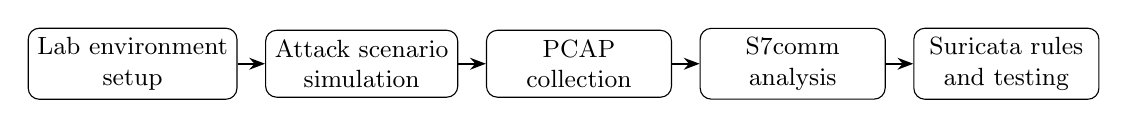
\begin{tikzpicture}[
        node distance=0.55cm and 0.35cm,
        box/.style={draw, rounded corners, align=center, font=\small,
            minimum width=2.35cm, minimum height=0.85cm},
        arr/.style={-{Stealth[length=2mm]}, thick}
    ]
        \node[box] (lab) {Lab environment\\setup};
        \node[box, right=of lab] (atk) {Attack scenario\\simulation};
        \node[box, right=of atk] (pcap) {PCAP\\collection};
        \node[box, right=of pcap] (ana) {S7comm\\analysis};
        \node[box, right=of ana] (ids) {Suricata rules\\and testing};
        \draw[arr] (lab) -- (atk);
        \draw[arr] (atk) -- (pcap);
        \draw[arr] (pcap) -- (ana);
        \draw[arr] (ana) -- (ids);
    \end{tikzpicture}
    \caption{Research methodology workflow of the thesis}
    \label{fig:methodology-flow}
\end{figure}

The scope of this chapter stops at traffic analysis and scenario description; writing Suricata rules and evaluating alert accuracy are presented in the next chapter.

\section{Experimental environment setup}
\label{sec:lab-setup}

\subsection{Deployment principles}

The lab environment is designed as a controlled simulation on virtual machines. All virtual machines are deployed using VMware LAN Segment objects (two LAN segments are used: 192.168.50.0/24 for the Controller Layer and 192.168.60.0/24 for the Superuser Layer). The IDS is deployed in passive mode by placing it in the same LAN segment. Figure~\ref{fig:lab-topology} shows how the two segments are connected and which hosts carry S7comm traffic in the default lab layout.

Because of how VMware vSwitch behaves like a conventional hub rather than a switch, placing the IDS in the same LAN segment and enabling promiscuous mode on the network interface is equivalent to a SPAN/mirror port on a physically deployed switch.

\begin{figure}[htbp]
    \centering
    
\includegraphics[width=0.95\textwidth]{Figure/lab_topology.png}
    \caption{Lab topology on VMware LAN Segments. \textbf{Controller Layer} (\texttt{192.168.50.0/24}): OpenPLC RUNTIME at \texttt{192.168.50.10}. \textbf{Superuser Layer} (\texttt{192.168.60.0/24}): FUXA EDITOR at \texttt{192.168.60.10}. A virtual router (\texttt{192.168.50.1}/\texttt{192.168.60.1}) routes between the segments. Black arrows: HMI Read Var request/response; red arrows: attacker Write Var and modified Read Var response (MITM scenario, Section~\ref{sec:stuxnet_mitm_sim}). The IDS VM (\texttt{172.16.16.7}) shares the Controller segment in promiscuous mode and is omitted from the diagram for clarity.}
    \label{fig:lab-topology}
\end{figure}

\subsection{Tools used}

OpenPLC is an open-source platform that simulates a physical PLC on a computer. The software runs on Windows, Linux, macOS, and Raspberry Pi. It supports control programs under the IEC 61131-3 standard and can connect to SCADA, HMI, or other industrial devices. OpenPLC has two main components:

- \href{https://autonomylogic.com/runtime}{OpenPLC Runtime}: the PLC engine that simulates a physical PLC. OpenPLC Runtime V4 supports several industrial protocols, including Siemens S7comm. When this protocol is enabled on OpenPLC Runtime V4, the runtime listens on port 102 and serves the Siemens S7comm protocol through the internal Snap7 driver. This thesis uses OpenPLC Runtime V4.

Figure~\ref{fig:S7_on_OpenPLC} shows S7comm enabled on OpenPLC Runtime V4.

\begin{figure}[htbp]
    \centering
    
\includegraphics[width=0.78\textwidth]{Figure/S7_on_OpenPLC.png}
    \caption{S7comm enabled on OpenPLC Runtime V4}
    \label{fig:S7_on_OpenPLC}
\end{figure}


- \href{https://autonomylogic.com/download}{OpenPLC Editor}: the IDE for writing programs for OpenPLC Runtime. It interacts with OpenPLC Runtime through a RESTful API on port 8443. In this thesis, it is used to write code, compile programs, load programs into the PLC, and debug programs. This thesis uses OpenPLC Editor V4.

Figure~\ref{fig:OpenPLC_Editor} shows openPLC Editor for writing, compiling, loading, and debugging programs.

\begin{figure}[htbp]
    \centering
    
\includegraphics[width=0.78\textwidth]{Figure/OpenPLC_Editor.png}
    \caption{OpenPLC Editor for writing, compiling, loading, and debugging programs}
    \label{fig:OpenPLC_Editor}
\end{figure}

FUXA (Docker \texttt{frangoteam/fuxa:snap7}, port 1881) is used to design and display the HMI interface. It is an open-source, web-based HMI that supports the Siemens S7comm protocol.

Figure~\ref{fig:FUXA} shows fUXA for designing and displaying the HMI interface.

\begin{figure}[htbp]
    \centering
    \includegraphics[width=0.78\textwidth]{Figure/FUXA.png}
    \caption{FUXA for designing and displaying the HMI interface}
    \label{fig:FUXA}
\end{figure}


Snap7 is an open-source library developed to connect to, transmit data with, and control automation devices. It is one of the most widely used open-source libraries in the automation industry.

Snap7 supports Siemens S7 communication protocols (S7comm) to connect and exchange data with Siemens automation devices. Its main features include:

\begin{itemize}
    \item Reading and writing variables in the PLC
    \item Accessing DB and OB blocks in the PLC
    \item Providing device status information
\end{itemize}

Characteristics of Snap7: 

\begin{itemize}
    \item Can be used with common programming languages such as C++, C\#, Python, and Java, allowing developers to choose the language best suited to their project. 
    \item Runs on multiple operating systems, including Windows, Linux, and macOS, which gives flexibility in application development.
    \item Compatible with many S7 PLC families and supports communication with S7-200, S7-300, S7-400, S7-1200, and S7-1500 PLCs, making integration into existing systems easier.
\end{itemize}

\subsection{Lab GUI tools}
\label{sec:lab-gui}

Running repeated experiments by hand---SSH into the Attacker VM to start a script, then SSH into the IDS VM to read Suricata logs---is slow and error-prone. Two desktop applications were therefore added as a thin control layer over the lab: they do not implement new attack logic; they provide a single window to trigger the same scenarios that are described later in this chapter and to observe the sensor response in real time.

\textbf{Attack Tool.} This client-side GUI is the operator console for generating S7comm traffic. The user sets the target PLC (address, rack, slot) and the remote Attacker host, then selects a scenario category from a fixed list---reconnaissance, process writes, denial of service, malformed packets, or Start/Stop replay---and starts execution with one click. The tool runs the corresponding script on the Attacker over SSH and streams command output into a log panel, so each run can be repeated without retyping commands. It only produces traffic; it does not display IDS alerts.

Figure~\ref{fig:demo-attack-recon} shows an example run: a reconnaissance scenario against the lab PLC, with live script output in the log area.

\begin{figure}[htbp]
    \centering
    
\includegraphics[width=0.82\textwidth]{Figure/Demo1.png}
    \caption{Attack Tool: scenario selection, PLC/Attacker settings, and live execution log.}
    \label{fig:demo-attack-recon}
\end{figure}

\textbf{Suricata Rules Tool.} This companion GUI connects to the IDS VM. It supports three operational views: browsing and editing the S7comm rule set, deploying validated rules to Suricata, and streaming new alerts as they are written to the sensor log. Network scope (\texttt{HOME\_NET}, capture interface) can be adjusted from the same window so rule tests match the lab topology in Figure~\ref{fig:lab-topology}.

Figure~\ref{fig:demo-rules-editor} shows the rule editor; Figure~\ref{fig:demo-rules-alerts} shows the live alert panel after a scenario has been triggered from the Attack Tool.

\begin{figure}[htbp]
    \centering
    
\includegraphics[width=0.82\textwidth]{Figure/Demo2.png}
    \caption{Suricata Rules Tool: rule list, metadata, and editable signature text.}
    \label{fig:demo-rules-editor}
\end{figure}

\begin{figure}[htbp]
    \centering
    
\includegraphics[width=0.82\textwidth]{Figure/Demo3.png}
    \caption{Suricata Rules Tool: live alert stream while attack traffic is mirrored to the IDS.}
    \label{fig:demo-rules-alerts}
\end{figure}

\textbf{Typical workflow.} Both tools are opened on the engineering workstation. The operator starts a scenario in the Attack Tool, then enables alert streaming in the Rules Tool. If Suricata lines appear while the script runs, the mirror path and rule deployment are working; detailed scenario behaviour and expected signatures are analysed in the attack sections below and in Chapter~\ref{sec:rules-by-scenario}.


\section{Attack scenarios and traffic analysis}
\label{sec:attack-scenarios}

The following sections describe the simulated scenarios in detail. 

\subsection{Reconnaissance}
\label{sec:reconnaissance}

Nmap is used with NSE scripts to discover devices in a network range. These scripts use S7comm-specific scanning techniques to avoid overloading devices in the OT network.

\begin{packetdump}
nmap -p 102 --script s7-info <IP_ADDRESS>
\end{packetdump}

Output:

\begin{packetdump}
ubuntu@ubuntuserver2204:~$ nmap -p 102 --script s7-info 192.168.50.0/24
Starting Nmap 7.80 ( https://nmap.org ) at 2026-04-21 16:23 UTC
Nmap scan report for 192.168.50.1
Host is up (0.0018s latency).

PORT    STATE  SERVICE
102/tcp closed iso-tsap

Nmap scan report for 192.168.50.10
Host is up (0.0027s latency).

PORT    STATE SERVICE
102/tcp open  iso-tsap
| s7-info:
|   Module: 6ES7 315-2EH14-0AB0
|   Basic Hardware: 6ES7 315-2EH14-0AB0
|   Version: 3.2.6
|   System Name: SNAP7-SERVER
|   Module Type: CPU 315-2 PN/DP
|   Serial Number: S C-C2UR28922012
|_  Copyright: Original Siemens Equipment
Service Info: Device: specialized

Nmap done: 256 IP addresses (2 hosts up) scanned in 3.21 seconds
\end{packetdump}


Nmap detected that host \texttt{192.168.50.10} is a virtual machine running OpenPLC Runtime with the S7 server enabled. It identified this device as a Siemens S7-300 series PLC. Analysis of packets captured during the scan shows the following process:


\begin{enumerate}

\item First, a TCP SYN scan to find devices in the network range:

Figure~\ref{fig:sreconnaissanceimage2png} shows TCP SYN scan to discover hosts in the network range.

\begin{figure}[htbp]
    \centering
    
\includegraphics[width=0.9\textwidth]{../attacks/reconnaissance/image-2.png}
    \caption{TCP SYN scan to discover hosts in the network range}
    \label{fig:sreconnaissanceimage2png}
\end{figure}


Two devices responded with RST packets with IP addresses ending in \texttt{.50.1} and \texttt{50.10}. Address \texttt{50.1} is the router gateway of the network range, and \texttt{50.10} is the IP of PLC 01. Traffic is filtered by these IP addresses.


\item Port 102 scan of \texttt{.50.10}


The stages of the scan can be divided as follows:



Figure~\ref{fig:sreconnaissanceimage5png} shows stages of the port 102 scan.

\begin{figure}[htbp]
    \centering
    
\includegraphics[width=0.9\textwidth]{../attacks/reconnaissance/image-5.png}
    \caption{Stages of the port 102 scan}
    \label{fig:sreconnaissanceimage5png}
\end{figure}



\begin{itemize}
    \item Establish a connection to TCP 102 using the TCP three-way handshake
    \item Establish COTP (Figure~\ref{fig:sreconnaissanceimage4png}).
\end{itemize}

\begin{figure}[htbp]
    \centering
    
\includegraphics[width=0.9\textwidth]{../attacks/reconnaissance/image-4.png}
    \caption{COTP connection establishment}
    \label{fig:sreconnaissanceimage4png}
\end{figure}


    The source here is 01, i.e., the workstation



    \item S7comm establishment


After COTP is established, the client sets up S7comm by sending an S7 \texttt{Setup communication} request with function code \texttt{0xF0} (packet 1046) to the PLC server and receives a response in packet 1047. 


Figure~\ref{fig:sreconnaissanceimage6png} shows S7comm communication setup.

\begin{figure}[htbp]
    \centering
    
\includegraphics[width=0.9\textwidth]{../attacks/reconnaissance/image-6.png}
    \caption{S7comm communication setup}
    \label{fig:sreconnaissanceimage6png}
\end{figure}


After S7 communication is established, both sides can exchange data using S7 commands. Here, the \texttt{Read SZL} command is used to read PLC status information. \texttt{Read SZL} is a subfunction in the CPU functions group of S7comm.


SZL is a virtual list that describes the current state of the PLC. The PLC does not store this list in advance; it is generated only when a client requests an SZL read. When the request is received, the PLC collects the current status of its components, packages them into an SZL data structure, and returns them to the client. The SZL list is 16 bits long with the following structure:


Figure~\ref{fig:sreconnaissanceimage8png} shows structure of the 16-bit SZL identifier.

\begin{figure}[htbp]
    \centering
    
\includegraphics[width=0.9\textwidth]{../attacks/reconnaissance/image-8.png}
    \caption{Structure of the 16-bit SZL identifier}
    \label{fig:sreconnaissanceimage8png}
\end{figure}



For example, in packet 1048:


\begin{packetdump}
S7 Communication
    Parameter: (Request) ->(CPU functions) ->(Read SZL)
        Parameter head: 0x000112
        Parameter length: 4
        Method (Request/Response): Req (0x11)
        0100 .... = Type: Request (4)
        .... 0100 = Function group: CPU functions (4)
        Subfunction: Read SZL (1)
        Sequence number: 0
    Data (SZL-ID: 0x0011, Index: 0x0001)
        Return code: Success (0xff)
        Transport size: OCTET STRING (0x09)
        Length: 4
        SZL-ID: 0x0011, Diagnostic type: CPU, Number of the partial list extract: All identification data records of a module, Number of the partial list: Module identification
            0000 .... .... .... = Diagnostic type: CPU (0x0)
            0000 0000 0001 0001 = Number of the partial list extract: All identification data records of a module (0x0011)
            .... .... 0001 0001 = Number of the partial list: Module identification (0x11)
        SZL-Index: 0x0001
\end{packetdump}


This request asks the PLC to return object management system status through the SZL read function. The read is requested at SZL-ID \texttt{0x0011} and Index \texttt{0x0001}. This part of the SZL returns \texttt{Diagnostic type: CPU, Number of the partial list extract}. Specifically:




\begin{packetdump}
Hex: 0x0011 =   0000    0000    00010001
                |       |       |
                |       |       +-- Which sub-list to retrieve,
                |       |           here Module Identification
                |       +-- Which part of that sub-list to retrieve;
                |           0 means the entire sub-list
                +-- Module class: CPU
\end{packetdump}


\begin{itemize}
    \item \texttt{Module class}: identifies the type of device to read
\end{itemize}


\begin{table}[H]
    \centering
    \footnotesize
    \begin{tabular}{|l|l|}
        \hline
        \textbf{Module class} & \textbf{Binary value} \\
        \hline
        CPU & 0000 \\
        \hline
        IM (Interface module) & 0100 \\
        \hline
        FM (Function module) & 1000 \\
        \hline
        CP (Communication processor) & 1100 \\
        \hline
    \end{tabular}
\end{table}


\begin{itemize}
    \item Some \texttt{Partial list number} types:
\end{itemize}


\begin{table}[H]
    \centering
    \footnotesize
    \begin{tabular}{|l|l|}
        \hline
        \textbf{Partial list type} & \textbf{Binary value} \\
        \hline
        Module Identification & 0001 0001 \\
        \hline
        CPU Characteristics & 0001 0010 \\
        \hline
        Module Status & 0001 0011 \\
        \hline
        Communication Status & 0001 1100 \\
        \hline
        Connection Status & 0001 1101 \\
        \hline
        Diagnostic Buffer & 0010 0010 \\
        \hline
        Diagnostic Status & 0010 0011 \\
        \hline
        Module list (rack)  (*extended*) & 0001 0001 0001 \\
        \hline
        Memory info & 0001 0011 0001 \\
        \hline
        Protection Level & 0010 0011 0010 \\
        \hline
    \end{tabular}
\end{table}


The PLC responds in packet 1049:


\begin{packetdump}
S7 Communication
    
    . . .
    Data (SZL-ID: 0x0011, Index: 0x0000)
        Return code: Success (0xff)
        Transport size: OCTET STRING (0x09)
        Length: 120
        SZL-ID: 0x0011, Diagnostic type: CPU, Number of the partial list extract: All identification data records of a module
        . . .
        SZL-Index: 0x0000
        SZL partial list length in bytes: 28
        SZL partial list count: 4

        SZL data tree (list count no. 1)
            Index: Identification of the module (0x0001)
            MlfB (Order number of the module): 6ES7 315-2EH14-0AB0 
            BGTyp (Module type ID): 0x00c0
            Ausbg (Version of the module or release of the operating system): 4
            Ausbe (Release of the PG description file): 1
\end{packetdump}


This packet returned the Module Identification value, corresponding to the \texttt{Module: 6ES7 315-2EH14-0AB0} field seen in the Nmap output.


Next, a read request is sent for SZL-ID \texttt{0x001c}, i.e., the \texttt{Communication Status} sub-list of module class \texttt{CPU}.


Figure~\ref{fig:sreconnaissanceimage7png} shows read SZL for Communication Status.

\begin{figure}[htbp]
    \centering
    
\includegraphics[width=0.9\textwidth]{../attacks/reconnaissance/image-7.png}
    \caption{Read SZL for Communication Status}
    \label{fig:sreconnaissanceimage7png}
\end{figure}


\begin{packetdump}
S7 Communication
    . . .
    Data (SZL-ID: 0x001c, Index: 0x0000)

        SZL-Index: 0x0000
        SZL partial list length in bytes: 34
        SZL partial list count: 10

        SZL data tree (list count no. 1)
            Index: Name of the automation system (0x0001)
            Name (Name of the PLC): SNAP7-SERVER
            Reserved: 0000000000000000

        SZL data tree (list count no. 2)
            Index: Name of the module (0x0002)
            Name (Name of the module): CPU 315-2 PN/DP
            Reserved: 0000000000000000

        SZL data tree (list count no. 3)
            Index: Plant designation of the module (0x0003)
            Tag (Plant identification of the module): 

        SZL data tree (list count no. 4)
            Index: Copyright entry (0x0004)
            Copyright: Original Siemens Equipment
            Reserved: 000000000000
        ...
\end{packetdump}


This packet returned the information shown in the Nmap output fields \texttt{Serial Number: S C-C2UR28922012}, \texttt{Version: 3.2.6}, \texttt{System Name: SNAP7-SERVER}, \texttt{Module Type: CPU 315-2 PN/DP}, and \texttt{Copyright: Original Siemens Equipment}.

\subsection{Scanning with other tools based on DCP}


DCP is a protocol in the PROFINET standard set. It is used to discover and configure devices on a PROFINET network. It is mainly used to connect to PLCs running on PROFINET before they can be assigned an IP address, because DCP operates at Layer 2 (Data Link), similar to ARP in TCP/IP. A DCP identify request is sent to discover devices on the network and wait for responses from those devices.


DCP can perform three main functions:

\begin{enumerate}
    \item Discovery: scan all devices connected on the same LAN.
\end{enumerate}


\begin{enumerate}
    \item Basic Configuration: assign IP address, subnet mask, gateway, and NameOfStation to a device.
\end{enumerate}


\begin{enumerate}
    \item Identification: request a specific device to blink its LED so its physical location in the electrical cabinet can be confirmed.
\end{enumerate}


There are several ways to scan PLC devices through DCP:


\begin{itemize}
    \item Open TIA Portal and run PLC discovery
    \item Use the Metasploit module auxiliary/scanner/scada/profinet\_siemens
    \item Use the script \textbackslash{}texttt\{SiemensScan.py\} (\url{./SiemensScan.py})
\end{itemize}


However, scanning OpenPLC with these methods in this project did not detect the PLC. This is because OpenPLC Runtime does not support DCP.


\subsection{Scanning PLC blocks}


After scanning PLC information, PLC blocks can be scanned to obtain information about control program blocks using Snap7 \texttt{.list\_blocks()} and \texttt{.list\_blocks\_of\_type(type)}. The script is available here (\url{./scanBlock.py}).


\begin{packetdump}
All blocks: <block list count OB: 0 FB: 0 FC: 0 SFB: 0 SFC: 0x0 DB: 2 SDB: 0>
\end{packetdump}


\begin{packetdump}
DB 1:
    Block type: 10
    Block number: 1
    Block language: 5
    Block flags: 1
    MC7Size: 128
    Load memory size: 220        
    Local data: 0
    SBB Length: 20
    Checksum: 0
    Version: 1
    Code date: b'1999/11/18'
    Interface date: b'1999/11/18'
    Author: b''
    Family: b''
    Header: b''

DB 2:
    Block type: 10
    Block number: 2
    Block language: 5
    Block flags: 1
    MC7Size: 128
    Load memory size: 220
    Local data: 0
    SBB Length: 20
    Checksum: 0
    Version: 1
    Code date: b'1999/11/18'
    Interface date: b'1999/11/18'

    Author: b''
    Family: b''
    Header: b''
\end{packetdump}


A PLC includes the following blocks:


\begin{itemize}
    \item \textbf{OB}: The main block for organizing the control program. Similar to \texttt{main () \{\}} in C++.
\end{itemize}


\begin{itemize}
    \item \textbf{(S)DB}: Contains data used by the control program. DB is a user-created data block; SDB is a system data block created by Siemens.
\end{itemize}


\begin{itemize}
    \item \textbf{(S)FC}: Contains reusable functions for the control program. FC is stateless: it does not store state and has no dedicated memory.
\end{itemize}


\begin{itemize}
    \item \textbf{(S)FB}: Similar to FC but stateful. It is usually linked to a DB to store its state.
\end{itemize}


However, due to OpenPLC Runtime simulation limits, only datablock \texttt{DB: 2} is shown even though the PLC is running a control program (in that case, the program OB would differ from 0).


Figure~\ref{fig:ksreconnaissanceimagepng} shows pLC block scan result.

\begin{figure}[htbp]
    \centering
    
\includegraphics[width=0.9\textwidth]{../attacks/reconnaissance/image.png}
    \caption{PLC block scan result}
    \label{fig:ksreconnaissanceimagepng}
\end{figure}


For each datablock, the following information is obtained:



\begin{packetdump}
DB 1:
    Block type: 10                   -> 10(decimal) = 0x0A(hex) = OB(block type)
    Block number: 1                  -> Block sequence number in the PLC (0x0001)
    Block language: 5                -> Block programming language (AWL, KOP, FUP, SCL, DB, GRAPH) (0x05)
    Block flags: 1                
    MC7Size: 128                     -> Size of readable/writable data area
    Load memory size: 220            -> Readable/writable data area + header/metadata 
    Local data: 0                    -> Stack data. DBs have no stack unlike logic blocks, so 0
    SBB Length: 20                   
    Checksum: 0                      -> Block checksum (0x00)
    Version: 1                       
    Code date: b'1999/11/18'         -> Block creation date (b'1999/11/18'). Error on virtual PLC simulation
    Interface date: b'1999/11/18'    -> Block update date (b'1999/11/18'). Error on virtual PLC simulation
    Author: b''                    
    Family: b''                      
    Header: b''                     
\end{packetdump}


\textit{See parameters in S7\_constants.txt (\url{../../docs/Report/S7_constants.txt}).}


Observe packets during block scanning:


Figure~\ref{fig:sreconnaissanceimage1png} shows S7 block scan traffic.

\begin{figure}[htbp]
    \centering
    
\includegraphics[width=0.9\textwidth]{../attacks/reconnaissance/image-1.png}
    \caption{S7 block scan traffic}
    \label{fig:sreconnaissanceimage1png}
\end{figure}


\begin{enumerate}
    \item Packets 13 and 14 initiate the S7 command connection
\end{enumerate}


\begin{enumerate}
    \item Packets 15 and 16 request the list of all blocks
\end{enumerate}


\begin{packetdump}
S7 Communication
    Header: (Userdata)
        Protocol Id: 0x32
        ROSCTR: Userdata (7)
        Redundancy Identification (Reserved): 0x0000
        Protocol Data Unit Reference: 256
        Parameter length: 8
        Data length: 4
    Parameter: (Request) ->(Block functions) ->(List blocks)
        Function: CPU services (0x00)
        Item count: 1
        Variable specification: 0x12
        Length of following address specification: 4
        Syntax Id: ParameterShort (0x11)
        01.. .... = Type: Request (1)
        ..00 0011 = Function group: Block functions (3)
        Subfunction: List blocks (1)
        Sequence number: 0
    Data
        Return code: Object does not exist (0x0a)
        Transport size: NULL (0x00)
        Length: 0
\end{packetdump}


This request belongs to \texttt{CPU services} > \texttt{Block functions} > \texttt{List blocks}. The response returns blocks in the PLC:


\begin{packetdump}
S7 Communication
    Header: (Userdata)
        Protocol Id: 0x32
        ROSCTR: Userdata (7)
    . . .
    Parameter: (Response) ->(Block functions) ->(List blocks)
        Function: CPU services (0x00)
        Item count: 1
        Variable specification: 0x12
        Length of following address specification: 8
        Syntax Id: ParameterExtended (0x12)
        10.. .... = Type: Response (2)
        ..00 0011 = Function group: Block functions (3)
        Subfunction: List blocks (1)
    . . .
    Data
        Return code: Success (0xff)
        Transport size: OCTET STRING (0x09)
        Length: 28
        \ldots
        Item [3]: (Block type FC)
            Block type: 0C (FC)
            Block count: 0
        Item [4]: (Block type DB)
            Block type: 0A (DB)
            Block count: 2
        Item [5]: (Block type SDB)
            Block type: 0B (SDB)
            Block count: 0
 \ldots
\end{packetdump}


\begin{enumerate}
    \item Packets 17 and 18 request information on available blocks, here \texttt{DB: 2}.
\end{enumerate}


\begin{enumerate}
    \item Packets 19 and 20 read information about DB1:
\end{enumerate}


\begin{packetdump}
S7 Communication
   ....
    Data [DB 1]
        Return code: Success (0xff)
        Transport size: OCTET STRING (0x09)
        Length: 8
        Block type: 0A (DB)
        Block number: 00001
        Filesystem: A (Active embedded module)
\end{packetdump}


Response:


\begin{packetdump}
S7 Communication
    . . .
    Data: (Block:[DB 1])
        Return code: Success (0xff)
        Transport size: OCTET STRING (0x09)
        Length: 78
        Block type: \x01 (Unknown Block type: 0x0100)
        Length of Info: 74
        Unknown blockinfo 2: 0x2200
        Constant 3: pp
        Unknown byte(s) blockinfo: 01
        0000 0001 = Block flags: 0x01, Linked
        Block language: DB (5)
        Subblk type: DB (10)
        Block number: 1
        Length load memory: 220
        Block Security: None (0)
        Code timestamp: Nov 18, 1999 00:00:00.000
        Interface timestamp: Nov 18, 1999 00:00:00.000
        SSB length: 20
        ADD length: 0
        Localdata length: 0
        MC7 code length: 128
        Author: 
        Family: 
        Name (Header): 
        Version (Header): 0.1
        Unknown byte(s) blockinfo: 00
        Block checksum: 0x0000
        Reserved 1: 0x00000000
        Reserved 2: 0x00000000
\end{packetdump}


This matches the information obtained from the \texttt{scanBlock.py} script.

\end{enumerate}


\subsection{4.3 Start/Stop PLC (Replay Attack)}
\label{sec:start_stop_plc}


This is a typical replay attack against a PLC: reusing captured S7comm packets from TIA Portal \texttt{Start CPU} / \texttt{Stop CPU} commands on S7-300, without additional authentication on the S7comm channel.

\subsubsection{Captured payload}


\begin{table}[H]
    \centering
    \footnotesize
    \begin{tabular}{|l|l|l|}
        \hline
        Command & Function code & Payload (hex) \\
        \hline
        Start CPU & \texttt{0x28} (PLC Control / PI-Service \texttt{P\_PROGRAM}) & \texttt{0300002502f0803201000005000014000028000000000000fd000009505f50524f4752414d} \\
        \hline
        Stop CPU & \texttt{0x29} (PLC Stop) & \texttt{0300002102f0803201000006000010000029000000000009505f50524f4752414d} \\
        \hline
    \end{tabular}
\end{table}

Packet structure for PLC Control and PLC Stop command groups:

\begin{packetdump}
    TPKT (4 Byte) + COTP DT (3 Byte) + S7 Header (10 Byte) + Parameter +  data PI-Service
\end{packetdump}
    
    
\begin{itemize}
    \item Start: \texttt{param\_length = 5}, function \texttt{0x28}, parameter block contains \texttt{0xfd} (RUN state) + name \texttt{P\_PROGRAM}.

Figure~\ref{fig:cksstartstopplcimage2png} shows start CPU S7comm packet.

\begin{figure}[htbp]
    \centering
    
\includegraphics[width=0.9\textwidth]{../attacks/start_stop_plc/image-2.png}
    \caption{Start CPU S7comm packet}
    \label{fig:cksstartstopplcimage2png}
\end{figure}


Figure~\ref{fig:cksstartstopplcimage3png} shows start CPU packet detail.

\begin{figure}[htbp]
    \centering
    
\includegraphics[width=0.9\textwidth]{../attacks/start_stop_plc/image-3.png}
    \caption{Start CPU packet detail}
    \label{fig:cksstartstopplcimage3png}
\end{figure}



\item Stop: \texttt{param\_length = 6}, function \texttt{0x29}.

Figure~\ref{fig:acksstartstopplcimagepng} shows stop CPU S7comm packet.

\begin{figure}[htbp]
    \centering
    
\includegraphics[width=0.9\textwidth]{../attacks/start_stop_plc/image.png}
    \caption{Stop CPU S7comm packet}
    \label{fig:acksstartstopplcimagepng}
\end{figure}


Figure~\ref{fig:cksstartstopplcimage1png} shows stop CPU packet detail.

\begin{figure}[htbp]
    \centering
    
\includegraphics[width=0.9\textwidth]{../attacks/start_stop_plc/image-1.png}
    \caption{Stop CPU packet detail}
    \label{fig:cksstartstopplcimage1png}
\end{figure}



\end{itemize}

\subsection{DoS attack on the S7comm channel}
\label{sec:dos_s7comm}

In OT environments, DoS aims to disrupt safe operation: the PLC cannot process control commands in time, the HMI loses data synchronization, or the engineering station cannot establish an S7 session. MITRE ATT\&CK for ICS classifies these behaviors under the Impact tactic, for example T0814 Denial of Service, T0803 Block Command Message, and T0804 Block Reporting Message.

Unlike web application DoS (HTTP flood), DoS against Siemens PLCs over Ethernet typically exploits TCP port 102 and the S7comm protocol:

\begin{enumerate}
    \item Connection resource exhaustion: open/close TCP connections to port 102 at high frequency (connection churn), or send many SYN packets, filling the session table on the PLC/S7 stack.
    \item Valid S7 command flood: repeat \texttt{Setup Communication} (\texttt{0xF0}), \texttt{Read SZL} (userdata CPU services), or \texttt{Read/Write Var}---syntactically valid payloads still load the CPU and processing queue.
    \item Reconnaissance abuse as a weapon: Read SZL / List Blocks at very high frequency serves both reconnaissance and service DoS (similar to excessive SCADA scanning).
\end{enumerate}

All three types are implemented in a single script, \texttt{attacks/dos/s7comm\_dos.py}. By default, \texttt{--mode all} runs three phases sequentially (\texttt{setup\_flood} $\rightarrow$ \texttt{tcp\_connect} $\rightarrow$ \texttt{szl\_flood}), each lasting about 10\,s with an 8\,s pause between phases so Suricata can record alerts before the next flood type (matching the \texttt{threshold} 10\,s window in \texttt{ics\_dos.rules}).

\begin{table}[H]
    \centering
    \footnotesize
    \begin{tabular}{|l|l|l|l|}
        \hline
        Phase (--mode all) & Description & Suricata rule & Default workers \\
        \hline
        1 -- \texttt{setup\_flood} & Repeated Setup Communication PDU on new TCP sessions & \texttt{1000041}, \texttt{1000043} & 4 \\
        \hline
        2 -- \texttt{tcp\_connect} & Fast connect/disconnect on :102 & \texttt{1000040} & 6 \\
        \hline
        3 -- \texttt{szl\_flood} & \texttt{read\_szl(0x0011)} via Snap7 & \texttt{1000042} & 2 \\
        \hline
    \end{tabular}
    \caption{S7comm DoS sequence in one script run (default)}
    \label{tab:dos-modes}
\end{table}

Lab deployment (single command):

\begin{packetdump}
python3 attacks/dos/s7comm_dos.py <IP_PLC>
# equivalent: --mode all --duration 10 --pause 8
\end{packetdump}

Each mode can be run separately with \texttt{--mode setup\_flood} (or \texttt{tcp\_connect}, \texttt{szl\_flood}) when analyzing PCAP per scenario.

Traffic is captured by Suricata on the IDS at the mirror interface. Detection uses \texttt{ics\_dos.rules} (\texttt{sid:1000040}--\texttt{1000043}): \texttt{threshold} with \texttt{track by\_src}, counting valid S7 packets within 10\,s---no malformed payload required. Thresholds should be tuned against the HMI baseline to avoid false positives.

\subsection{PLC Program Upload and Download}
\label{sec:down_up_program}

In Siemens terminology, the meaning is opposite to common IT usage:


\begin{itemize}
    \item Download: the master/client sends the control program to the slave PLC. This corresponds to loading code in TIA Portal.
\end{itemize}


\begin{itemize}
    \item Upload: the master/client retrieves the control program from the PLC.
\end{itemize}


The control program source and most program data are stored as blocks. Block types in Siemens devices include:


\begin{itemize}
    \item \textbf{OB}: The main block for organizing the control program. Similar to \texttt{main () \{\}} in C++.
\end{itemize}


\begin{itemize}
    \item \textbf{(S)DB}: Contains data used by the control program. DB is a user-created data block; SDB is a system data block created by Siemens.
\end{itemize}


\begin{itemize}
    \item \textbf{(S)FC}: Contains reusable functions for the control program. FC is stateless: it does not store state and has no dedicated memory.
\end{itemize}


\begin{itemize}
    \item \textbf{(S)FB}: Similar to FC but stateful. It is usually linked to a DB to store its state.
\end{itemize}



\subsubsection{Upload}


\begin{packetdump}
%%{init: {'sequence': {'messageMargin': 60}} }%%
sequenceDiagram
    participant Workstation
    participant PLC

    Workstation->>PLC: Job - Start Upload: Block Address
    PLC->>Workstation: Ack Data - Start Upload: Block Length

    Workstation-->>PLC: Job - Upload Block
    PLC-->>Workstation: Ack Data - Upload Block: Block Data

    Workstation->>PLC: Job - End Upload
    PLC->>Workstation: Ack Data - End Upload
\end{packetdump}


\begin{enumerate}
    \item Start Upload: The client sends a command requesting the control program the PLC is running (\textcolor{blue}{Job} Start Upload), and the PLC responds to that request (\textcolor{green}{ACK} Start Upload). This command includes the following fields in order:
\end{enumerate}


\begin{table}[H]
    \centering
    \footnotesize
    \begin{tabular}{|l|l|l|}
        \hline
        Field & \textcolor{blue}{Job} Start Upload & \textcolor{green}{ACK} Start Upload \\
        \hline
        \texttt{Function Code} (1 byte) & Fixed \texttt{0x1d} & Same \\
        \hline
        \texttt{Function Status} (1 byte) & - & - \\
        \hline
        Unknown (2 bytes) & \texttt{0x0000} & \texttt{0x0100} \\
        \hline
        \texttt{Session ID} (4 bytes) & - & Identifier for each upload session, returned by the PLC and used in subsequent commands throughout the upload session \\
        \hline
        Context-dependent name & \texttt{Filename Length} (1 byte) followed by \texttt{Filename} specifying the block to retrieve & \texttt{Length String Length} (1 byte) followed by \texttt{Length String}, a decimal value indicating the block length the PLC will return in the data field of the next response packet \\
        \hline
    \end{tabular}
\end{table}


    \texttt{Filename} identifies a block as follows:


\begin{packetdump}
    ------------------------------------------------------------------------------------------------------------------
    |  1 char - File identifier  |  2 chars - Block type | 5 chars - Block number | 1 char - Destination file system |
    ------------------------------------------------------------------------------------------------------------------
\end{packetdump}


    Where:


\begin{itemize}
    \item \texttt{File identifier} is always \texttt{\_}
    \item \texttt{Block type} is one of the block types listed above
\end{itemize}


\begin{table}[H]
    \centering
    \footnotesize
    \begin{tabular}{|l|l|}
        \hline
        Hex & Block type \\
        \hline
        0x08 & OB \\
        \hline
        0x0a & DB \\
        \hline
        0x0b & SDB \\
        \hline
        0x0c & FC \\
        \hline
        0x0d & SFC \\
        \hline
        0x0e & FB \\
        \hline
        0x0f & SFB \\
        \hline
    \end{tabular}
\end{table}


\begin{itemize}
    \item \texttt{Block number} is the block identifier
    \item \texttt{Destination file system} includes \texttt{A} for the active file system or \texttt{P} for the passive file system. Blocks copied to the active file system run immediately when the PLC operates; blocks copied to the passive file system must be activated before execution.
\end{itemize}


    For example, \texttt{\_0800001P} is OB block number 1 copied to the passive file system.


\begin{enumerate}
    \item Upload Block: After receiving Start Upload, the client sends Upload Block to request a control program data block. The PLC returns that block in the response data field. This command includes the following fields in order:
\end{enumerate}


\begin{table}[H]
    \centering
    \footnotesize
    \begin{tabular}{|l|l|l|}
        \hline
        Field & \textcolor{blue}{Job} Upload Block & \textcolor{green}{ACK} Upload Block \\
        \hline
        \texttt{Function Code} (1 byte) & Fixed \texttt{0x1e} & Same \\
        \hline
        \texttt{Function Status} (1 byte) & - & \texttt{0x01} if more blocks remain to upload, \texttt{0x00} if no blocks remain \\
        \hline
        Unknown (2 bytes) & \texttt{0x0000} & \texttt{0x0000} \\
        \hline
        \texttt{Session ID} (4 bytes) & Uses existing sessionID & Same \\
        \hline
        \texttt{Data} & - & Contains the control program code, including \texttt{Length} (2 bytes) for this data section, fixed \texttt{0x00fb}, and \texttt{Block Data} holding the block to upload. This data is in ASCII format \\
        \hline
    \end{tabular}
\end{table}


\begin{enumerate}
    \item End Upload: After receiving all data according to the \texttt{Length String} field in the ACK Start Upload packet, the client sends End Upload to close the upload session. The PLC responds to confirm the session ended successfully. This command includes the following fields in order:
\end{enumerate}


\begin{table}[H]
    \centering
    \footnotesize
    \begin{tabular}{|l|l|l|}
        \hline
        Field & \textcolor{blue}{Job} End Upload & \textcolor{green}{ACK} End Upload \\
        \hline
        \texttt{Function Code} (1 byte) & Fixed \texttt{0x1f} & Same \\
        \hline
    \end{tabular}
\end{table}


\subsubsection{Download}


\begin{packetdump}
%%{init: {'sequence': {'messageMargin': 60}} }%%
sequenceDiagram
    participant Workstation
    participant PLC

    Workstation->>PLC: Job - Request Download: Block Address, Length
    PLC->>Workstation: Ack Data - Request Download
    
  
    PLC-->>Workstation: Job - Download Block: Block Address
    Workstation-->>PLC: Ack Data - Download Block: Block Data

    Workstation->>PLC: Job - Download Ended
    PLC->>Workstation: Ack Data - Download Ended
\end{packetdump}


\begin{enumerate}
    \item \textbf{Start Download}: The client sends a command to request that the PLC prepare to receive a new control program (\textcolor{blue}{Job} Request Download), and the PLC responds to that request (\textcolor{green}{ACK} Request Download). The \textcolor{blue}{Job} Request Download packet adds two fields: \texttt{Block Length}, which indicates the length of the data block the client will send, and \texttt{Payload Length}, which works similarly but does not include the block header length.
\end{enumerate}



\begin{enumerate}
    \item \textbf{Download Block}: The PLC proactively sends a request asking the client to send a data block of the new control program. The client sends that data block in the data section of the response packet.
\end{enumerate}


The remaining fields are identical to those in the Upload section. One note during Download: \texttt{Session ID} is always \texttt{0x00000000} and is not used; instead, Download uses \texttt{Filename} to identify items within a Download session.


\subsection{Traffic simulation}


In this section, we attempted to simulate downloading and uploading PLC control programs but were unsuccessful due to limitations of the simulation software.


When uploading program code from OpenPLC Editor to OpenPLC Runtime, the program is sent through the OpenPLC Runtime RESTful API rather than using the standard S7comm structure.


Figure~\ref{fig:ksdownupprogramimage5png} shows uploading a program from OpenPLC Editor to OpenPLC Runtime via RESTful API.

\begin{figure}[htbp]
    \centering
    
\includegraphics[width=0.9\textwidth]{../attacks/down_up_program/image-5.png}
    \caption{Uploading a program from OpenPLC Editor to OpenPLC Runtime via RESTful API}
    \label{fig:ksdownupprogramimage5png}
\end{figure}


OpenPLC Runtime does not support loading programs in the usual Siemens S7comm way.


Another approach is to simulate program upload on a Siemens PLC through PLC Sim Advance. In this approach, the program is sent using the standard S7comm structure.


Step 1: Set up a virtual switch for Siemens virtual devices to use:


Figure~\ref{fig:ksdownupprogramimage2png} shows virtual switch setup for Siemens virtual devices.

\begin{figure}[htbp]
    \centering
    
\includegraphics[width=0.9\textwidth]{../attacks/down_up_program/image-2.png}
    \caption{Virtual switch setup for Siemens virtual devices}
    \label{fig:ksdownupprogramimage2png}
\end{figure}


Step 2: Run a Siemens PLC in PLC Sim Advance on the same network as the virtual switch. However, PLC Sim Advance only supports simulating Siemens S7-1500 PLCs.


Figure~\ref{fig:cksdownupprogramimagepng} shows siemens PLC running in PLC Sim Advance.

\begin{figure}[htbp]
    \centering
    
\includegraphics[width=0.9\textwidth]{../attacks/down_up_program/image.png}
    \caption{Siemens PLC running in PLC Sim Advance}
    \label{fig:cksdownupprogramimagepng}
\end{figure}


Step 3: Connect the PLC to an HMI WinCC through an IE general connection card


Figure~\ref{fig:ksdownupprogramimage1png} shows pLC connected to HMI WinCC via IE general connection card.

\begin{figure}[htbp]
    \centering
    
\includegraphics[width=0.9\textwidth]{../attacks/down_up_program/image-1.png}
    \caption{PLC connected to HMI WinCC via IE general connection card}
    \label{fig:ksdownupprogramimage1png}
\end{figure}


Step 4: Create a PLC program, download it to the PLC, and run a test:


Figure~\ref{fig:ksdownupprogramimage3png} shows pLC program in running mode with PLC Sim Advance and HMI WinCC.

\begin{figure}[htbp]
    \centering
    
\includegraphics[width=0.9\textwidth]{../attacks/down_up_program/image-3.png}
    \caption{PLC program in running mode with PLC Sim Advance and HMI WinCC}
    \label{fig:ksdownupprogramimage3png}
\end{figure}


The screenshot shows the PLC program in running mode, the PLC running in PLC Sim Advance, and HMI WinCC displaying PLC variable values.


However, when observing packets in Wireshark, Wireshark could not parse S7comm packets. After investigation, this is because S7-1500 uses the S7comm plus protocol and there is no way to force S7-1500 to use standard S7comm (according to this article (\url{https://industrialmonitordirect.com/blogs/knowledgebase/s7comm-vs-s7comm-plus-switching-protocol-in-s7-1500-hmi-communication}), enabling the option \texttt{Permit access with PUT/GET communication from remote partners} only provides compatibility so other machines can read information from S7comm plus as if it were standard S7comm; Wireshark still cannot parse S7comm plus packets.


Figure~\ref{fig:ksdownupprogramimage6png} shows wireshark unable to parse S7comm plus packets.

\begin{figure}[htbp]
    \centering
    
\includegraphics[width=0.9\textwidth]{../attacks/down_up_program/image-6.png}
    \caption{Wireshark unable to parse S7comm plus packets}
    \label{fig:ksdownupprogramimage6png}
\end{figure}


Figure~\ref{fig:ksdownupprogramimage4png} shows wireshark identifying only the outer COTP layer of S7comm plus packets.

\begin{figure}[htbp]
    \centering
    
\includegraphics[width=0.9\textwidth]{../attacks/down_up_program/image-4.png}
    \caption{Wireshark identifying only the outer COTP layer of S7comm plus packets}
    \label{fig:ksdownupprogramimage4png}
\end{figure}


Wireshark can only identify the COTP layer on the outside of S7comm plus packets and cannot parse the S7comm plus packet wrapped inside this COTP packet.



Therefore, in this project we will use simulated traffic from the following page: https://wiki.wireshark.org/S7comm

\subsection{Stuxnet attack simulation (MITM)}
\label{sec:stuxnet_mitm_sim}

\paragraph{Historical attack chain.}

\begin{enumerate}
    \item \textbf{Windows infection:} Stuxnet entered internal networks via USB and spread using Windows zero-days, reporting to C\&C servers~\cite{falliere2010stuxnet,stuxnet_work_details}.
    \item \textbf{Step~7 hooking (*):} On each infected workstation it hooked \texttt{s7otbxdx.dll} to intercept and modify traffic between Step~7 and the PLC---a software-layer man-in-the-middle attack (Figures~\ref{fig:stuxnet_mitm_sim-image-9} and~\ref{fig:stuxnet_mitm_sim-image-10}).
    \item \textbf{Centrifuge control interference:} Stuxnet modified PLC logic to raise centrifuge speed above safe limits. Malicious code was injected via Step~7, executed on the PLC, forwarded to the variable frequency drive (VFD), and physically damaged the centrifuge while falsified values were sent to WinCC.
\end{enumerate}

\begin{figure}[htbp]
    \centering
    
\includegraphics[width=0.85\textwidth]{../attacks/stuxnet_mitm_sim/image-9.png}
    \caption{Normal Step~7--PLC communication}
    \label{fig:stuxnet_mitm_sim-image-9}
\end{figure}

\begin{figure}[htbp]
    \centering
    
\includegraphics[width=0.85\textwidth]{../attacks/stuxnet_mitm_sim/image-10.png}
    \caption{Stuxnet MITM on Step~7--PLC link}
    \label{fig:stuxnet_mitm_sim-image-10}
\end{figure}



Stuxnet activated only when the target PLC and drive matched narrow criteria: Siemens S7-300, Vacon or Fararo Paya drives, and operating frequency between 807~Hz and 1210~Hz---typical of gas centrifuges rather than ordinary industrial equipment. When matched, it stepped output frequency through levels such as 1410~Hz, 2~Hz, and 1064~Hz to damage the process while concealing the effect on monitoring data.

\textit{In this thesis, the same operational outcome is reproduced at the S7comm network layer (Figure~\ref{fig:lab-topology}) rather than via DLL hooking as in the historical campaign.}

(*) \textit{TIA Portal bundles STEP~7, WinCC, PLCSIM, and drive configuration tools for Siemens S7 PLC families.}

\paragraph{Attack simulation.}

The lab reproduces the same \emph{operational} outcome as the historical campaign---change what the PLC executes while keeping the operator display unchanged---but implements it on the wire rather than inside Step~7 libraries. The scenario therefore has three layers that must be prepared before the attack runs: a PLC program that exposes the process variables of interest, an HMI that polls those variables over S7comm, and an attacker host that can both write the PLC and sit on the HMI--PLC path. The subsections below describe each layer; the attacker stage then combines an unauthorized write, ARP redirection, and in-flight editing of Read~Var responses.

\subsubsection{PLC setup}

The scenario control program is imported into OpenPLC Editor from the project bundle supplied with the lab. Because OpenPLC allows only one data type per datablock, inputs and outputs are split across DB1 and DB2 (Figure~\ref{fig:stuxnet_mitm_sim-image-1}). Structured Text logic drives simulated motor speed oscillating around setpoint \texttt{iSetpoint = 1200} (Figure~\ref{fig:stuxnet_mitm_sim-image-2}).

\begin{figure}[htbp]
    \centering
    
\includegraphics[width=0.85\textwidth]{../attacks/stuxnet_mitm_sim/image-1.png}
    \caption{OpenPLC datablocks DB1 and DB2}
    \label{fig:stuxnet_mitm_sim-image-1}
\end{figure}

\begin{figure}[htbp]
    \centering
    
\includegraphics[width=0.85\textwidth]{../attacks/stuxnet_mitm_sim/image-2.png}
    \caption{Structured Text tags and logic}
    \label{fig:stuxnet_mitm_sim-image-2}
\end{figure}

The tags used later in traffic analysis are \texttt{iSimSpeed} and \texttt{iSetpoint} in DB1 (16-bit words), \texttt{iCounter} for the oscillation pattern, and \texttt{bCentrifugeStatus} in DB2 (0 = normal, 1 = overspeed above 1500~Hz). Once compiled and loaded, the runtime serves these variables on TCP/102 like a Siemens CPU.

\subsubsection{HMI setup}

The supervisory project is imported into FUXA and bound to the same PLC tags (Figure~\ref{fig:stuxnet_mitm_sim-image-8}). Under normal operation the HMI shows speed near 1200 in green, consistent with the OpenPLC debugger (Figure~\ref{fig:stuxnet_mitm_sim-image-17}). The program must remain loaded in the runtime before the HMI connects; otherwise polling will fail or show stale values.

\begin{figure}[htbp]
    \centering
    
\includegraphics[width=0.85\textwidth]{../attacks/stuxnet_mitm_sim/image-8.png}
    \caption{FUXA project import and tags}
    \label{fig:stuxnet_mitm_sim-image-8}
\end{figure}

\begin{figure}[htbp]
    \centering
    
\includegraphics[width=0.85\textwidth]{../attacks/stuxnet_mitm_sim/image-17.png}
    \caption{OpenPLC Editor debugger view}
    \label{fig:stuxnet_mitm_sim-image-17}
\end{figure}

During steady-state polling, HMI--PLC traffic repeats two Read~Var request--response pairs: a 4-byte read of \texttt{iSimSpeed} and \texttt{iSetpoint} in DB1 (Figures~\ref{fig:stuxnet_mitm_sim-image-4} and~\ref{fig:stuxnet_mitm_sim-image-5}), and a 1-byte read of \texttt{bCentrifugeStatus} in DB2 (Figures~\ref{fig:stuxnet_mitm_sim-image-6} and~\ref{fig:stuxnet_mitm_sim-image-7}). Multi-byte values appear little-endian in the captures (\texttt{iSimSpeed} = \texttt{0x042d} $\rightarrow$ 1069; \texttt{iSetpoint} = \texttt{0x04b0} $\rightarrow$ 1200). These captures establish the baseline against which the MITM stage is compared.

\begin{figure}[htbp]
    \centering
    
\includegraphics[width=0.85\textwidth]{../attacks/stuxnet_mitm_sim/image-4.png}
    \caption{Read Var request: DB1 variables}
    \label{fig:stuxnet_mitm_sim-image-4}
\end{figure}

\begin{figure}[htbp]
    \centering
    
\includegraphics[width=0.85\textwidth]{../attacks/stuxnet_mitm_sim/image-5.png}
    \caption{Read Var response: DB1 variables}
    \label{fig:stuxnet_mitm_sim-image-5}
\end{figure}

\begin{figure}[htbp]
    \centering
    
\includegraphics[width=0.85\textwidth]{../attacks/stuxnet_mitm_sim/image-6.png}
    \caption{Read Var request: status tag}
    \label{fig:stuxnet_mitm_sim-image-6}
\end{figure}

\begin{figure}[htbp]
    \centering
    
\includegraphics[width=0.85\textwidth]{../attacks/stuxnet_mitm_sim/image-7.png}
    \caption{Read Var response: normal status}
    \label{fig:stuxnet_mitm_sim-image-7}
\end{figure}

\subsubsection{Attacker stage}

With PLC and HMI running normally, the attacker host executes three coordinated actions. Step~1 changes the physical setpoint on the PLC; step~2 forces HMI-bound traffic through the attacker; step~3 restores the old setpoint only in responses destined for the HMI. Steps~2 and~3 must be active before step~1 matters to the operator display, but all three run concurrently in the lab script.

\begin{enumerate}
    \item \textbf{Unauthorized write.} From the attacker workstation, a Snap7 or Python S7comm client opens a session to the PLC and issues \texttt{Write Var} on \texttt{DB1.DBW2} (\texttt{iSetpoint}), changing the value from 1200 to 2000. No credential or session binding is required on classic S7comm~\cite{inprotech_s7comm_security}; possession of network reachability and memory addressing is sufficient.

    \item \textbf{ARP spoofing.} Bettercap poisons the ARP cache between the supervisory subnet gateway (\texttt{192.168.60.1}) and the HMI (\texttt{192.168.60.10}) in full-duplex mode so both HMI$\rightarrow$PLC and PLC$\rightarrow$HMI legs traverse the attacker before reaching their true destination.

    \item \textbf{Response forgery.} Packets redirected to the attacker are handed to a Linux NFQUEUE handler. The handler parses each S7comm \texttt{Ack\_Data} Read~Var response and rewrites \texttt{iSetpoint} from 2000 back to 1200 before reinjecting the frame toward the HMI.
\end{enumerate}

After the write alone (without steps~2--3), debugger and HMI both reflect the new setpoint. The packet dump below contrasts nominal operation with the post-write state:

\begin{packetdump}
    Current Speed  | Setpoint Speed    | Centrifuge Status
    --------------------------------------------------
    b'\x03\xc1'    |    b'\x04\xb0'    |    b'\x00'
    b'\x07\xe4'    |    b'\x07\xd0'    |    b'\x01'
\end{packetdump}

Here \texttt{iSetpoint} moves from \texttt{0x04b0} to \texttt{0x07d0} and \texttt{bCentrifugeStatus} becomes~1 because simulated speed exceeds 1500~Hz. Without MITM, the HMI trend turns red around 2000 (Figure~\ref{fig:stuxnet_mitm_sim-image-14}) and Wireshark shows the updated setpoint in PLC$\rightarrow$HMI traffic (Figure~\ref{fig:stuxnet_mitm_sim-image-15}).

\begin{figure}[htbp]
    \centering
    
\includegraphics[width=0.55\textwidth]{../attacks/stuxnet_mitm_sim/image-14.png}
    \caption{HMI view without MITM}
    \label{fig:stuxnet_mitm_sim-image-14}
\end{figure}

\begin{figure}[htbp]
    \centering
    
\includegraphics[width=0.85\textwidth]{../attacks/stuxnet_mitm_sim/image-15.png}
    \caption{Wireshark: updated setpoint in traffic}
    \label{fig:stuxnet_mitm_sim-image-15}
\end{figure}

When ARP spoofing and response forgery are enabled together with the write, Wireshark on the HMI segment shows S7comm frames interleaved with spoofing traffic (Figure~\ref{fig:stuxnet_mitm_sim-image-13}). The operator screen still displays setpoint~1200 and nominal colouring (Figure~\ref{fig:stuxnet_mitm_sim-image-18}), while forwarded \texttt{Ack\_Data} payloads carry the forged word \texttt{0x04b0} (Figure~\ref{fig:stuxnet_mitm_sim-image-28}). The overspeed status byte may still read~1 in a separate response (Figure~\ref{fig:stuxnet_mitm_sim-image-29}), so concealment is partial rather than complete. The OpenPLC debugger, which is not on the spoofed path, continues to show execution near the written value of 2000 (Figure~\ref{fig:stuxnet_mitm_sim-image-3}).

\begin{packetdump}
    set arp.spoof.targets 192.168.60.1, 192.168.60.10
    set arp.spoof.internal true
    set arp.spoof.fullduplex true
    arp.spoof on
\end{packetdump}

\begin{figure}[htbp]
    \centering
    
\includegraphics[width=0.85\textwidth]{../attacks/stuxnet_mitm_sim/image-13.png}
    \caption{S7comm and ARP spoofing packets interleaved}
    \label{fig:stuxnet_mitm_sim-image-13}
\end{figure}

\begin{figure}[htbp]
    \centering
    
\includegraphics[width=0.55\textwidth]{../attacks/stuxnet_mitm_sim/image-18.png}
    \caption{HMI view with MITM: nominal setpoint display}
    \label{fig:stuxnet_mitm_sim-image-18}
\end{figure}

\begin{figure}[htbp]
    \centering
    
\includegraphics[width=0.85\textwidth]{../attacks/stuxnet_mitm_sim/image-28.png}
    \caption{Wireshark: forged setpoint field}
    \label{fig:stuxnet_mitm_sim-image-28}
\end{figure}

\begin{figure}[htbp]
    \centering
    
\includegraphics[width=0.85\textwidth]{../attacks/stuxnet_mitm_sim/image-29.png}
    \caption{Wireshark: overspeed status byte}
    \label{fig:stuxnet_mitm_sim-image-29}
\end{figure}

\begin{figure}[htbp]
    \centering
    
\includegraphics[width=0.85\textwidth]{../attacks/stuxnet_mitm_sim/image-3.png}
    \caption{OpenPLC debugger at actual speed}
    \label{fig:stuxnet_mitm_sim-image-3}
\end{figure}

In summary, the operator sees nominal setpoint 1200 on FUXA while the PLC debugger confirms logic running against the attacker-written value near 2000---the same deception pattern Stuxnet achieved through Step~7 hooks, reproduced here at the network layer.

\subsubsection{Attack analysis}

Network-layer forgery differs from DLL hooking because the attacker must parse and rewrite complete Ethernet frames at line rate. Bettercap alone is insufficient: its script interface cannot host a full S7comm parser, so the lab combines ARP redirection with the Linux NFQUEUE framework. Before queuing, the attacker enables IP forwarding, relaxes reverse-path filtering, adds a route to the PLC subnet, and installs \texttt{iptables} rules that copy TCP/102 flows into NFQUEUE. A userspace handler then receives each copied packet, validates the TPKT/COTP/S7 envelope, and either forwards unchanged or edits selected fields.

To know \emph{which} bytes to edit, the handler must understand Read~Var layout. An S7 PDU on TCP/102 stacks TPKT, COTP, an S7 header, and Param/Data sections (Figure~\ref{fig:iemensS7protocolstackpng}). Figures~\ref{fig:stuxnet_mitm_sim-image-19} and~\ref{fig:stuxnet_mitm_sim-image-20} show the framing layers; Figures~\ref{fig:stuxnetmitmsimimage25png} and~\ref{fig:stuxnetmitmsimimage26png} show representative Job and Ack\_Data Read~Var exchanges. The S7 header begins with protocol id~\texttt{0x32}; byte~8 (\texttt{ROSCTR}) distinguishes Job (\texttt{0x01}), Ack (\texttt{0x02}), and Ack\_Data (\texttt{0x03}).

\begin{figure}[htbp]
    \centering
    
\includegraphics[width=0.9\textwidth]{../attacks/stuxnet_mitm_sim/Siemens_S7_protocol_stack.png}
    \caption{Siemens S7 protocol stack}
    \label{fig:iemensS7protocolstackpng}
\end{figure}

\begin{figure}[htbp]
    \centering
    
\includegraphics[width=0.9\textwidth]{../attacks/stuxnet_mitm_sim/image-19.png}
    \caption{TPKT header}
    \label{fig:stuxnet_mitm_sim-image-19}
\end{figure}

\begin{figure}[htbp]
    \centering
    
\includegraphics[width=0.9\textwidth]{../attacks/stuxnet_mitm_sim/image-20.png}
    \caption{COTP header}
    \label{fig:stuxnet_mitm_sim-image-20}
\end{figure}

\begin{figure}[htbp]
    \centering
    
\includegraphics[width=0.9\textwidth]{../attacks/stuxnet_mitm_sim/image-25.png}
    \caption{Read Var request (Job PDU)}
    \label{fig:stuxnetmitmsimimage25png}
\end{figure}

\begin{figure}[htbp]
    \centering
    
\includegraphics[width=0.9\textwidth]{../attacks/stuxnet_mitm_sim/image-26.png}
    \caption{Read Var response (Ack\_Data PDU)}
    \label{fig:stuxnetmitmsimimage26png}
\end{figure}

In the Param section of a Read~Var Job, function code~\texttt{0x04} is followed by an item count and one or more request items. This lab uses Any-type addressing (\texttt{Syntax ID = 0x10}) throughout (Figures~\ref{fig:stuxnet-anytype-struct} and~\ref{fig:stuxnetmitmsimimage22png})~\cite{gmiru_s7comm_part2}. In the corresponding Ack\_Data message, each request item is replaced by a response item that adds return code~\texttt{0xff} and the payload word or byte read from the PLC (Figures~\ref{fig:stuxnet-readvar-response} and~\ref{fig:stuxnet_mitm_sim-image-23}). DB-Type and symbolic addressing are not used in this scenario; Figure~\ref{fig:stuxnetmitmsimimage24png} shows the DB-Type layout for comparison only.

\begin{figure}[htbp]
    \centering
    
\includegraphics[width=0.85\textwidth]{Figure/AnyTypeStruct.png}
    \caption{Any-type Read Var Param structure}
    \label{fig:stuxnet-anytype-struct}
\end{figure}

\begin{figure}[htbp]
    \centering
    
\includegraphics[width=0.9\textwidth]{../attacks/stuxnet_mitm_sim/image-22.png}
    \caption{Any-type addressing in captured traffic}
    \label{fig:stuxnetmitmsimimage22png}
\end{figure}

\begin{figure}[htbp]
    \centering
    
\includegraphics[width=0.9\textwidth]{../attacks/stuxnet_mitm_sim/image-21.png}
    \caption{Any-type request item fields}
    \label{fig:stuxnetmitmsimimage21png}
\end{figure}

\begin{figure}[htbp]
    \centering
    
\includegraphics[width=0.85\textwidth]{Figure/ReadVarResponse.png}
    \caption{Read Var response Data item structure}
    \label{fig:stuxnet-readvar-response}
\end{figure}

\begin{figure}[htbp]
    \centering
    
\includegraphics[width=0.9\textwidth]{../attacks/stuxnet_mitm_sim/image-23.png}
    \caption{Read Var response data item}
    \label{fig:stuxnet_mitm_sim-image-23}
\end{figure}

\begin{figure}[htbp]
    \centering
    
\includegraphics[width=0.9\textwidth]{../attacks/stuxnet_mitm_sim/image-24.png}
    \caption{DB-Type request and response items}
    \label{fig:stuxnetmitmsimimage24png}
\end{figure}

Wireshark dissects Param headers reliably but does not always expand Read~Var \emph{Data} payloads to individual tag values. No complete open-source decoder was available for the response layout used here, so the lab reimplemented the field walk described in~\cite{s7_parser_github} as a Python module and checked the output against Wireshark's partial decode (Figure~\ref{fig:stuxnetmitmsimimage16png}). That parser identifies the 29-byte Ack\_Data response that carries both \texttt{iSimSpeed} and \texttt{iSetpoint}; the intercept handler modifies only bytes~27--28 (the setpoint word), recalculates checksums, and reinjects the frame. Editing must keep pace with FUXA polling: a long poll interval delays visible updates even when forgery succeeds (Figure~\ref{fig:stuxnetmitmsimimage27png}).

\begin{figure}[htbp]
    \centering
    
\includegraphics[width=0.9\textwidth]{../attacks/stuxnet_mitm_sim/image-16.png}
    \caption{S7 packet parsed in Wireshark}
    \label{fig:stuxnetmitmsimimage16png}
\end{figure}

\begin{figure}[htbp]
    \centering
    
\includegraphics[width=0.9\textwidth]{../attacks/stuxnet_mitm_sim/image-27.png}
    \caption{FUXA HMI polling configuration}
    \label{fig:stuxnetmitmsimimage27png}
\end{figure}


\setcounter{subsubsection}{0}

\subsection{Sending malformed packets to the PLC}
\label{sec:malformed_plc}

Malformed packets (syntactically or semantically invalid packets) on the S7comm channel target the parser and protocol stack on the PLC or CP, rather than sending valid control commands at high frequency as in DoS (Section~\ref{sec:dos_s7comm}). In practice and in ICS fuzzing documentation, attackers often send PDUs with length fields that do not match the payload, invalid S7 headers, or Job/Userdata parameters with missing bytes---to cause temporary denial of service, close TCP/102 sessions, or (in rare cases) exploit memory bugs on weaker stacks.

This thesis does not aim to cover every infinite fuzz variant. Instead, it systematizes representative malformed groups commonly encountered when pentesting or fuzzing S7comm, then selects one or two representative samples per group to build lab payloads and corresponding Suricata rules (\texttt{detect/rules/s7comm\_malformed.rules}).

\paragraph{Four commonly used malformed groups.}

\begin{enumerate}
    \item Group 1---Encapsulation (TPKT / COTP): errors at the ISO-on-TCP layer before S7 processing. Examples: TPKT version other than \texttt{0x03}; TPKT \emph{length} field (bytes 2--3) declared larger or smaller than the actual TCP payload; COTP not a standard Data TPDU \texttt{02 F0 80}. The stack usually stops early and cannot parse the Job.
    \item Group 2---S7 header: TPKT/COTP may look valid, but the Protocol ID byte $\neq$ \texttt{0x32} or \texttt{ROSCTR} is not in the valid set (\texttt{0x01} Job, \texttt{0x02} Ack, \texttt{0x03} Ack\_Data, \texttt{0x07} Userdata). This is the layer for which Chapter~\ref{sec:detection-overview} uses offsets 7--8 for opcode rules.
    \item Group 3---Function layer (Job / parameters): a valid S7 header (\texttt{32 01}) but a nonexistent function code (e.g.\ \texttt{0xFF}) or a \texttt{Write Var} PDU (\texttt{0x05}) that is too short and lacks the item structure---the PLC returns a parameter error (similar to codes \texttt{0x0112}, \texttt{0xD801} in S7 documentation).
    \item Group 4---Truncation: sending only the beginning of a PDU (e.g.\ Setup Communication) without enough bytes to reach the function offset (\texttt{17}). This is a common ``missing-byte'' malformed pattern in random fuzzing or when a proxy truncates packets.
\end{enumerate}

\paragraph{Representative samples selected for the lab.}

Table~\ref{tab:malformed-phases} lists sample payloads, scripts, and Suricata \texttt{sid} values. Each sample starts from a valid Setup Communication PDU (same hex as \texttt{s7comm\_dos.py}) and modifies only one field (or truncates) so students can compare easily in Wireshark.

\begin{table}[H]
    \centering
    \footnotesize
    \begin{tabular}{|l|l|l|l|}
        \hline
        Group & \texttt{--mode} script & Change vs.\ valid Setup & SID \\
        \hline
        1 & \texttt{tpkt\_bad\_version} & TPKT byte 0 = \texttt{0x02} & 1000050 \\
        \hline
        1 & \texttt{tpkt\_len\_gt\_payload} & TPKT length = \texttt{0x0100}, body $\approx$ 36 B & 1000051 \\
        \hline
        1 & \texttt{tpkt\_len\_lt\_payload} & TPKT length = \texttt{0x0008}, full Setup body & 1000058 \\
        \hline
        1 & \texttt{cotp\_invalid} & Replace \texttt{02 F0 80} with \texttt{01 00 00} & 1000056 \\
        \hline
        2 & \texttt{s7\_bad\_protocol\_id} & Byte 7 = \texttt{0x31} & 1000052 \\
        \hline
        2 & \texttt{s7\_bad\_rosctr} & Byte 8 = \texttt{0xFF} & 1000053 \\
        \hline
        3 & \texttt{job\_bad\_opcode} & Byte 17 = \texttt{0xFF} (instead of \texttt{0xF0}) & 1000054 \\
        \hline
        3 & \texttt{write\_var\_malformed} & Job \texttt{0x05}, 20 B PDU (missing item) & 1000057 \\
        \hline
        4 & \texttt{setup\_truncated} & Send only the first 14 bytes & 1000055 \\
        \hline
    \end{tabular}
    \caption{Representative malformed samples and detection rule mapping}
    \label{tab:malformed-phases}
\end{table}

\paragraph{Script deployment.}

All scenarios are implemented in \texttt{attacks/malformed/s7comm\_malformed.py}. By default, \texttt{--mode all} runs 9 phases sequentially; each phase sends \texttt{--repeats} times (default 3) on a new TCP session to port 102, then waits \texttt{--pause} seconds (default 6) before the next phase---similar to DoS but without flooding: the goal is to produce clear malformed alerts in \texttt{fast.log}.

\begin{packetdump}
python3 attacks/malformed/s7comm_malformed.py <IP_PLC>
# equivalent to: --mode all --repeats 3 --pause 6
python3 attacks/malformed/s7comm_malformed.py <IP_PLC> --mode s7_bad_rosctr
\end{packetdump}

Processing on the wire: attacker $\rightarrow$ TCP/102 $\rightarrow$ mirror $\rightarrow$ Suricata. Unlike \texttt{ics\_dos.rules}, malformed rules do not use thresholds: each packet matching an anomalous signature may generate one alert (\texttt{sid:1000050}--\texttt{1000058}).

\paragraph{Expected behavior on the lab PLC and limitations.}

On simulated OpenPLC / S7 servers, the samples above usually lead to connection refusal, timeout, or TCP closure---rarely changing RUN/STOP state as in Start/Stop replay. Real Siemens PLCs typically have more robust stacks; this thesis treats malformed traffic as a means to detect anomalous behavior on the network, not as confirmed RCE exploitation. Some rules (e.g.\ \texttt{1000050} for invalid TPKT version) may trigger on non-S7 traffic on port 102; in the lab, narrow \texttt{HOME\_NET} and run scripts only against test PLCs.




\end{document}

